%% SECTION HEADER /////////////////////////////////////////////////////////////////////////////////////
\section{Damage indices}
\label{sec:di}

%% SECTION CONTENT ////////////////////////////////////////////////////////////////////////////////////
In the dissertation, several damage indices are analysed in the time - and frequency - domain. All of them are considered in two options, the entire length of the signal and the first wave package arrived at the sensor.
The packaged is extracted by windowing the full-length signals of the sensor  with a flattened Gaussian window in the form:
\begin{eqnarray}
	g(t)= \mathrm{exp}\left(-\left(\frac{t-t_0}{w_g}\right) ^{n}\right),
	\label{eq:psi_g}
\end{eqnarray}
where \(t_0\) is the center and \(w_g=0.5N_c/f_c\) is a half-width of the window, and n determines the slope of the window.

The following time-domain indices are take into consideration: \ac{p2p}, \ac{rmsd}, \ac{eng} in two kind.

\begin{eqnarray}
		\mathrm{P2P} & = & (A - A_0);\\
		\mathrm{RMSD} & = & \sqrt{\int{\left[\Psi(t)-\Psi_0(t)\right]^2\diff 		t/\int{\left[\Psi_0(t)\right]^2\diff t}}};\\
		\mathrm{ENG^1} & = & \left(\int{\left|\Psi(t)-\Psi_0(t)\right|^2\diff 	t/\int{\left|\Psi(t)\right|^2\diff t}}\right);\\
		\mathrm{ENG^2} & = & \left(\int{\left|\Psi_0(t)\right|^2\diff 	t/\int{\left|\Psi(t)\right|^2\diff t}}\right).
\end{eqnarray}

%\begin{figure}[!tbh]
%	\begin{center}
%		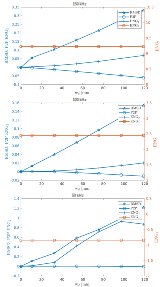
\includegraphics{Chapter_7/DI_I_W_f}
%	\end{center}
%	\caption{DIIWf}
%	\label{fig:DIIWf}
%\end{figure}
%\begin{figure}[!tbh]
%	\begin{center}
%		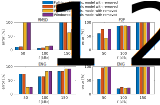
\includegraphics{Chapter_7/bar_f}
%	\end{center}
%	\caption{Bar}
%	\label{fig:bar_f}
%\end{figure}
%
%\begin{figure}[!tbh]
%	\begin{center}
%		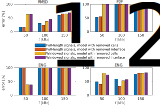
\includegraphics{Chapter_7/bar_h}
%	\end{center}
%	\caption{Bar}
%	\label{fig:bar_h}
%\end{figure}
